% arara: xelatex
\documentclass[11pt]{article} % размер шрифта
\usepackage{libertine}

\usepackage{tikz} % картинки в tikz
\usepackage{microtype} % свешивание пунктуации

\usepackage{array} % для столбцов фиксированной ширины

\usepackage{indentfirst} % отступ в первом параграфе

\usepackage{multicol} % текст в несколько колонок
\usepackage{verbatim}

\usepackage{csquotes}

\graphicspath{{images/}} % путь к картинкам

\usepackage{sectsty} % для центрирования названий частей
\allsectionsfont{\centering} % приказываем центрировать все sections

\usepackage{amsmath, amssymb} % куча стандартных математических плюшек

\usepackage[top=1cm, left=1cm, right=1cm, bottom=1cm]{geometry} % размер текста на странице

\usepackage{lastpage} % чтобы узнать номер последней страницы

\usepackage{enumitem} % дополнительные плюшки для списков
%  например \begin{enumerate}[resume] позволяет продолжить нумерацию в новом списке
\usepackage{caption} % подписи к картинкам без плавающего окружения figure

\usepackage{circuitikz} % для рисовки электрических цепей

\usepackage{physics} 

\usepackage{fancyhdr} % весёлые колонтитулы
\pagestyle{empty}
%\lhead{ФМТ}
%\chead{}
%\rhead{КЛШ-2019}
%\lfoot{}
%\cfoot{}
%\rfoot{\thepage/\pageref{LastPage}}
%\renewcommand{\headrulewidth}{0.4pt}
%\renewcommand{\footrulewidth}{0.4pt}



\usepackage{todonotes} % для вставки в документ заметок о том, что осталось сделать
% \todo{Здесь надо коэффициенты исправить}
% \missingfigure{Здесь будет картина Последний день Помпеи}
% команда \listoftodos — печатает все поставленные \todo'шки

\usepackage{booktabs} % красивые таблицы
% заповеди из документации:
% 1. Не используйте вертикальные линии
% 2. Не используйте двойные линии
% 3. Единицы измерения помещайте в шапку таблицы
% 4. Не сокращайте .1 вместо 0.1
% 5. Повторяющееся значение повторяйте, а не говорите "то же"

\usepackage{fontspec} % поддержка разных шрифтов
\usepackage{polyglossia} % поддержка разных языков

\setmainlanguage{russian}
\setotherlanguages{english}

\setmainfont{UbuntuMono Nerd Font Mono} % font name in archlinux
% \setmainfont{UbuntuMono Nerd Font} 

\usepackage{unicode-math}
\setmathfont{Fira Math} % выбираем шрифт
% можно также попробовать Helvetica, Arial, Cambria и т.Д.
% перешли на \usepackage{libertine}

% чтобы использовать шрифт Linux Libertine на личном компе,
% его надо предварительно скачать по ссылке
% http://www.linuxlibertine.org/

% \newfontfamily{\cyrillicfonttt}{Linux Libertine O}
% пояснение зачем нужно шаманство с \newfontfamily
% http://tex.stackexchange.com/questions/91507/

\AddEnumerateCounter{\asbuk}{\russian@alph}{щ} % для списков с русскими буквами
\setlist[enumerate, 2]{label=\asbuk*),ref=\asbuk*} % списки уровня 2 будут буквами а) б) ...


% делаем короче интервал в списках
\setlength{\itemsep}{0pt}
\setlength{\parskip}{0pt}
\setlength{\parsep}{0pt}


%%% В СЛЕДУЮЩЕЙ СТРОКЕ НУЖНО ПОПРАВИТЬ КРАТКОЕ НАЗВАНИЕ ТУРА:
\newcommand{\shortname}{ФМТ: Свалка} % тут каждый раз меняем на новый тур

% судейский экземляр выглядит так:
% заголовок \HeaderDiscussionMain или \HeaderGameMain
% анекдот \anecdote или напоминалка правил \judgenotes (анекдот при обсуждении, напоминалка правил в игре)
% задачи с решениями \MainTables или \TopTables

% школьный экземпляр выглядит так:
% заголовок \putlogo
% задачи без решения \MainTables или \TopTables

% всё это варьируется на основные столы (Main) и топ-столы (Top)


%%% СКОРЕЕ ВСЕГО ЭТИ ЧЕТЫРЕ СТРОКИ ПРАВИТЬ НЕ НАДО
\newcommand{\HeaderDiscussionMain}{\textbf{TOP SECRET!!! Сдай листок или съешь его!!!} \hspace*{1cm} \textbf{\shortname} \hspace*{1cm} \textbf{Разбор задач. Обычные столы.}}
\newcommand{\HeaderDiscussionTop}{\textbf{TOP SECRET!!! Сдай листок или съешь его!!!} \hspace*{1cm} \textbf{\shortname} \hspace*{1cm} \textbf{Разбор задач. top-3 столы.}}
\newcommand{\HeaderGameMain}{\textbf{TOP SECRET!!! Судейский экземпляр!!!} \hspace*{1cm} \textbf{\shortname} \hspace*{1cm} \textbf{Обычные столы}}
\newcommand{\HeaderGameTop}{\textbf{TOP SECRET!!! Судейский экземпляр!!!} \hspace*{1cm} \textbf{\shortname} \hspace*{1cm} \textbf{top-3 столы}}


% анекдот используется только судьями и только при обсуждении
% МОЖНО РАССКАЗАТЬ НОВЫЙ АНЕКДОТ
\newcommand{\anecdote}{Рубрика \textbf{анекдот} тура
    \begin{small}
    \begin{displayquote} 
        % \it Британские ученые выяснили, что если оттянуть яйца до колен, то в первую очередь порвутся голосовые связки.
    \end{displayquote}
    \end{small} % сюда пишем анекдот
}

% заметки используются только судьями и входят в игровой экземпляр
% МОЖНО НАПИСАТЬ КРАТКОЕ НАПУТСТВИЕ СУДЬЯМ НА ИГРУ
\newcommand{\judgenotes}{
    За одну итерацию оппонирования можно получить максимум 1 балл. 
    Вольные стрелки приносят команде от 0 до 3 баллов. 
    Штрафы за выход за три минуты при решении своей задачи: от 0 до 30 секунд — 1 балл штрафа, 
    от 30 до 60 секунд — 2 балла штрафа и далее 3 балла штрафа.
    Вольные стрелки не могут заявлять одну задачу более одного раза.
}



\newcommand{\putlogo}{
\begin{center}
\begin{tabular}{cc}

\includegraphics[scale=0.25]{klsh_logo.pdf} &
\raisebox{1cm}{
    {\Large\bf \shortname \hspace*{8cm} КЛШ $50$}
}
\end{tabular}
\end{center}
}

%%% ПРАВИМ СОДЕРЖИМОЕ ЗАДАЧ НИЖЕ ЭТОЙ ЛИНИИ:
\newcommand{\mathA}{
Ламзин купил квартиру с номером 400 в многоэтажной новостройке не на первом этаже. 
В каждом подъезде одинаковое количество этажей. 
На каждом этаже одинаковое количество квартир (больше одной, но меньше десяти). 
Потом застройщик поменял порядок нумерации подъездов, справа налево вместо исходного порядка слева направо, 
поэтому квартира Ламзина теперь имеет номер 323. 

В каком подъезде и на каком этаже теперь живёт Ламзин?
}

\newcommand{\mathAsol}{
Подъезд номер 5, 3-й этаж.

Неверный ответ в старой нумерации, ставим 2 балла: подъезд номер 6, 3-й этаж. 

Неверный ответ, если перепутать число этажей и число квартир на этаже, ставим 2 балла: подъезд номер 5, 2-й этаж.
}

\newcommand{\mathB}{
Роберт Гринштейн построил четырёхугольник $ABCD$ с $\angle ABD = \angle ACD = 45^{\circ}$, $\angle BAC = 30^{\circ}$ и $BC = 1$.

Переняв мудрость главного судьи ФМТ, найди $AD$.
}

\newcommand{\mathBsol}{
Углы соответствуют дугам $60^{\circ}$ и $90^{\circ}$. 
Радиус окружности равен $R = 1$, сторона квадрата равна $AD = \sqrt{2}$.

Если не увеличить угол в два раза, то получится $R = 1/\sqrt{2 - \sqrt{3}}$ и $AD = \sqrt{2 - \sqrt{2}}/\sqrt{2 - \sqrt{3}}$, ставим 1 балл. 
}

\newcommand{\physB}{
    \begin{minipage}{0.45\linewidth}
        Найди ток текущий через резистор имени Марины Хмельницкой, отмеченный шишкой, в цепи, спаянной Вовой Федоровым в виде фразы \textbf{"IDV-4:5"}, если на клеммы $A$ и $B$ подано напряжение $U = 85$ В. Сопротивление $R$ каждого резистора равно $1$ Ом.
    \end{minipage}\hfill
    \begin{minipage}{0.55\linewidth}
        \centering{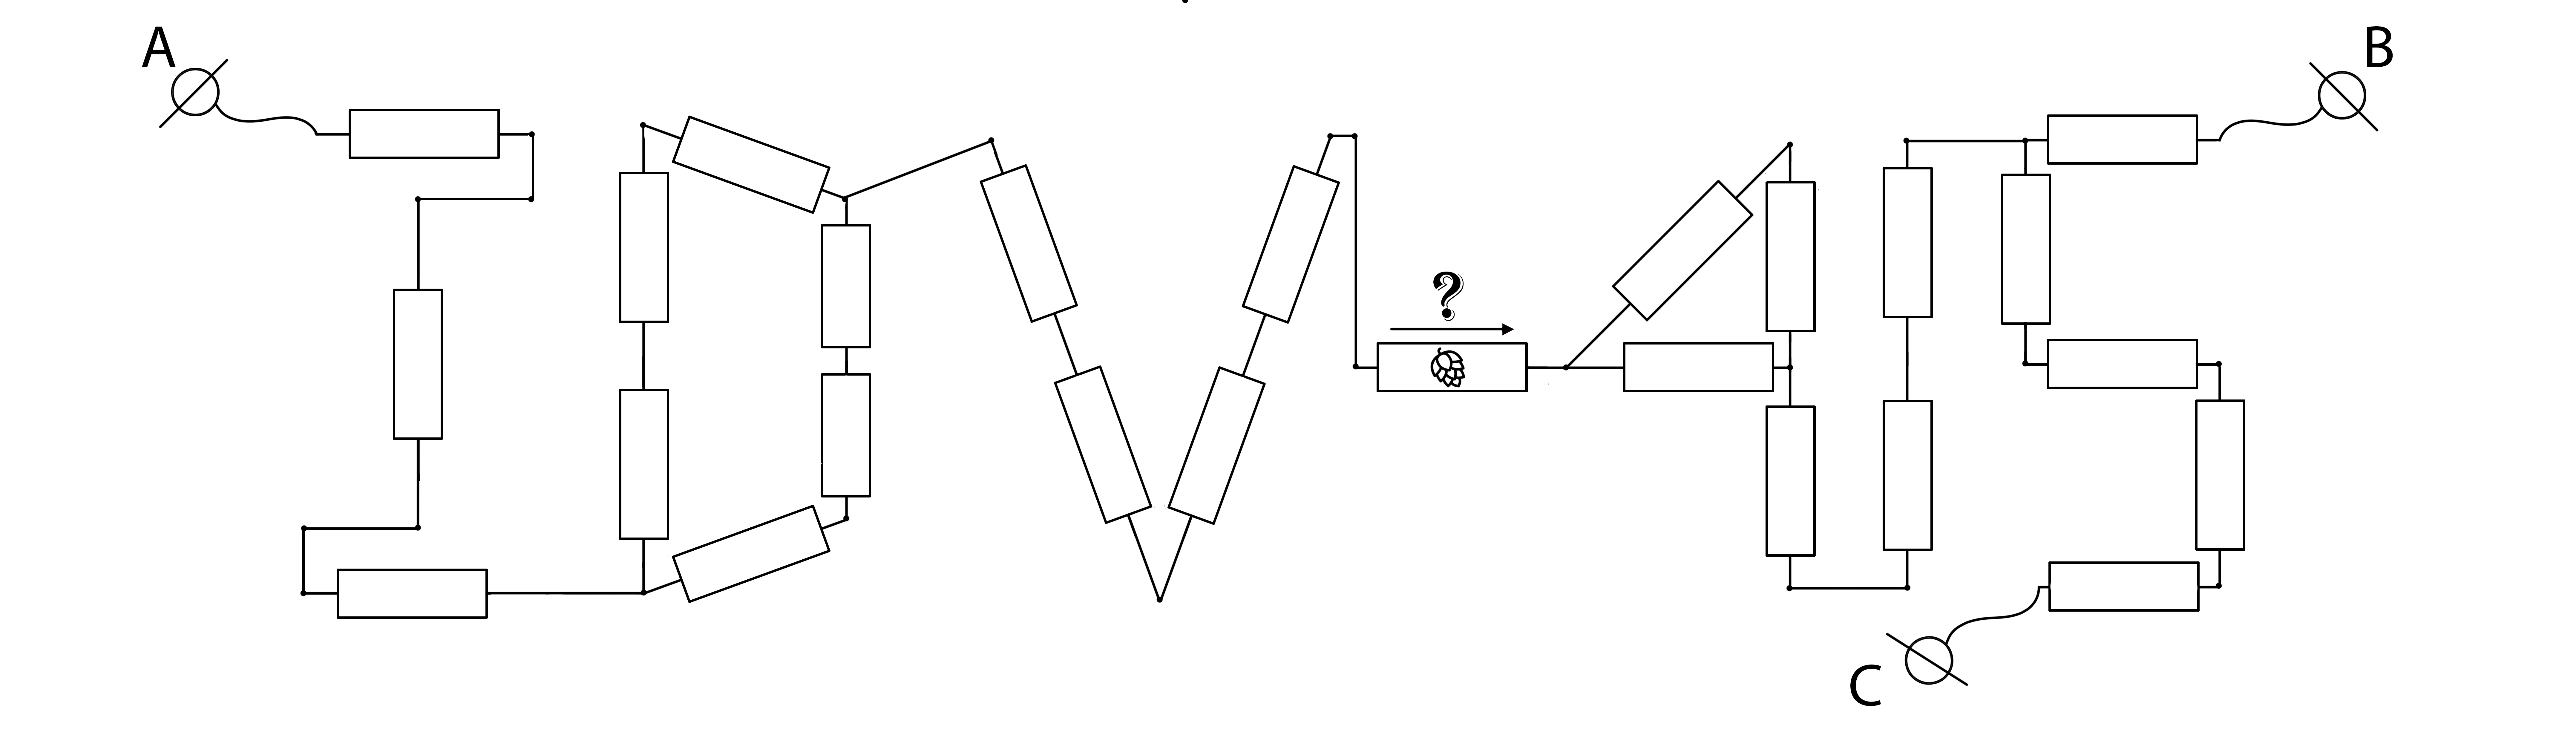
\includegraphics[width=\linewidth]{idv_4-5.jpg}}
    \end{minipage}
}   

\newcommand{\physBsol}{

    Эквивалентное сопротивление
    \begin{equation*}
        R_0 = 3R + 1.5R + 5R + 2/3R + 4R = (27/2 + 2/3)R = 85/6 R
    \end{equation*}

    Сила тока $I = \frac{U}{R_0} = 6$ А

    Ответ: $6$ А

    1 балл - посчитали с пятеркой; 2 балла - арифметическая ошибка
}

\newcommand{\physA}{
    \textbf{свалка, 2011 год (36 сезон)} На столе лежит квадратная книга массы $m$ и стороной длины $l$. Какую минимальную работу нужно совершить, чтобы раскрыть её на середине? Толщина книги много меньше $l$, ускорение свободного падения $g$.
}

\newcommand{\physAsol}{
    Нужно поднять половинку $m/2$ вертикально. Минимальная работа равна изменению потенциальной энергии центра масс 
    \begin{equation*}
        A_{min} = \frac{m}{2} g \frac{l}{2} = \frac{mgl}{4}
    \end{equation*}

    Ответ: $\frac{mgl}{4}$

    2 балл - не поделили массу/сторону на два
}
%%% ПРАВИМ КОМПОНОВКУ ТУРА НИЖЕ ЭТОЙ ЛИНИИ:

\newcommand{\MainTables}{
\begin{enumerate}
\item \mathA

\mathAsol
\item \mathB

\mathBsol
\item \physA

\physAsol
\item \physB

\physBsol
\end{enumerate}
}

\newcommand{\TopTables}{
\begin{enumerate}
\item \mathC

\mathCsol
\item \mathD

\mathDsol
\item \physA

\physAsol
\item \physC

\physCsol
\end{enumerate}
}

%%% НИЖЕ ЭТОЙ ЛИНИИ СКОРЕЕ ВСЕГО НИЧЕГО ПРАВИТЬ НЕ НАДО

\begin{document}

\HeaderDiscussionMain % судейский экземпляр для обсуждения обычных столов

\begin{small}
    \anecdote
\end{small}

\MainTables

\newpage

\HeaderDiscussionMain % судейский экземпляр для обсуждения обычных столов

\begin{small}
    \anecdote
\end{small}

\MainTables

\newpage

% \HeaderDiscussionTop % судейский экземпляр для обсуждения ТОП столов
% % может содержать анекдоты и прочий ограниченный контент

% \begin{small}
%     \anecdote
% \end{small}

% \TopTables

\newpage

% \HeaderDiscussionTop % судейский экземпляр для обсуждения ТОП столов

% \begin{small}
%     \anecdote
% \end{small}

% % \TopTables

\newpage

\HeaderGameMain % судейский экземпляр на игру обычных столов
% утечка после игры возможна, хотя и нежелательна

\begin{small}
    \judgenotes
\end{small}

\MainTables

\newpage % судейский экземпляр на игру ТОП столов
% утечка после игры возможна, хотя и нежелательна

% \HeaderGameTop

% \begin{small}
%     \judgenotes
% \end{small}

% \TopTables


%% школьные экземпляры... 
% зануляем решения :)
\renewcommand{\mathAsol}{}
\renewcommand{\mathBsol}{}
% \renewcommand{\mathCsol}{}
% \renewcommand{\mathDsol}{}
\renewcommand{\physAsol}{}
\renewcommand{\physBsol}{}
% \renewcommand{\physCsol}{}
% \renewcommand{\physDsol}{}


\newpage % школьный экземпляр обычных столов
\putlogo

\MainTables

\vspace{1pt}

\putlogo

\MainTables

% \newpage %% школьный экземпляр top3 столов

% \putlogo

% \TopTables

% \vspace{3.5pt}
% \putlogo

% \TopTables

\newcommand{\protocol}[2]{
\putlogo

{\Large Команда: #1 \hspace*{2cm} Судья: #2
}
\vspace*{1cm}

\begin{tabular}{ | p{2cm} | p{4cm} | p{4cm} |}
    \hline
    Задача & Время заявки & Балл \\
    \hline
    1 & &  \\ [2.1cm]
    \hline
    2 & &  \\ [2.1cm]
    \hline
    3 & &  \\ [2.1cm]
    \hline
    4 & &  \\ [2.1cm]
    \hline
\end{tabular}
\vspace*{0.5cm}

\begin{itemize}
    \item Судья! Первым делом фиксируй время заявки задачи в протоколе и на отдельной бумажке.
    \item Запиши на бумажку команду, время и балл за задачу. Продублируй информацию в протокол. Передай бумажку ласточке. 
    \item Задачи заявляют письменно.
    \item Каждую задачу можно заявить только один раз. 
    \item При сомнениях после получения решения можно попросить команду дать письменный дополнительный комментарий к решению.
    Не злоупотребляй этим.    
\end{itemize}


Начисление баллов:

\begin{itemize}
    \item если задача решена на 0 баллов или не заявлена к окончанию тура, команда получает 1200 штрафных секунд = 20 штрафных минут;
    \item если задача заявлена через $T$ секунд от начала и решена на $b>0$ баллов, команда получает $T/b$ штрафных секунд.
\end{itemize}

}


\newpage
\protocol{$\alpha$}{Тима Спрыжков}

\newpage
\protocol{$\beta$}{Паша Рябенко}

\newpage
\protocol{$\gamma$}{Настя Судницына}

\newpage
\protocol{$\delta$}{Андрей Трегубович}

\newpage
\protocol{$\eta$}{Роберт Гринштейн}

\newpage
\protocol{$\theta$}{Саша Акантьев}

\newpage
\protocol{$\varepsilon$}{Ян Шапиро}

\newpage
\protocol{$\lambda$}{Вова Федоров}

\newpage
\protocol{$\kappa$}{Марина Хмельницкая}

\newpage
\protocol{$\mu$}{Егор Лунёв}

\newpage
\protocol{$\nu$}{Андрей Трегубович}

\newpage
\protocol{$o$}{Герман Злобин}

\newpage
\protocol{$\pi$}{Саша Тимошков}
 
\newpage
\protocol{$\rho$}{Рома Лисин}

\newpage
\protocol{$\sigma$}{Никита Терентьев, Ярослав Федулов}

\newpage
\protocol{$\phi$}{Влада Синицына}

\newpage
\protocol{$\psi$}{Миша Красков}

\newpage
\protocol{$\chi$}{Вова Носков}

\newpage
\protocol{$\xi$}{Лев Назаров}

\newpage
\protocol{$\iota$}{Егор Скурковин, Артем Майдуров}

\newpage
\protocol{$\tau$}{Ваня Адо}

\newpage
\protocol{$\omega$}{Денис Гохфельд}

% резерв: Федулов, Торишн, Фонарева, Казаринова


\end{document}